\section{Evaluation}
\label{sec:eval}

\subsection{Dataset}
\label{subsec:dataset}
We collect two different datasets to show the usage of \textit{TransLayer}. One dataset is a control experiment that reproduces the RRC inference algorithm from~\cite{3g_rrc}, called \emph{Control Dataset}. The duration for \emph{Control Dataset} is 5 hours. Another dataset is collected from real-time web browsing in WCDMA network for an hour, called \emph{Browsing Dataset}.  We have evaluate the percentage of mapping in \S~\ref{subsec:cross-layer.mapping}, uniqueness analysis in \S~\ref{subsec:uniqueness.analysis}, and IP fragmentation and replication elimination in \S~\ref{subsec:ip.frag.and.dup} using \emph{Browsing Dataset}.

\subsection{Case Study}
\label{subsec:case.study}
\subsubsection{Abnormal RRC State Transition}

\begin{figure}[t!]
\centering
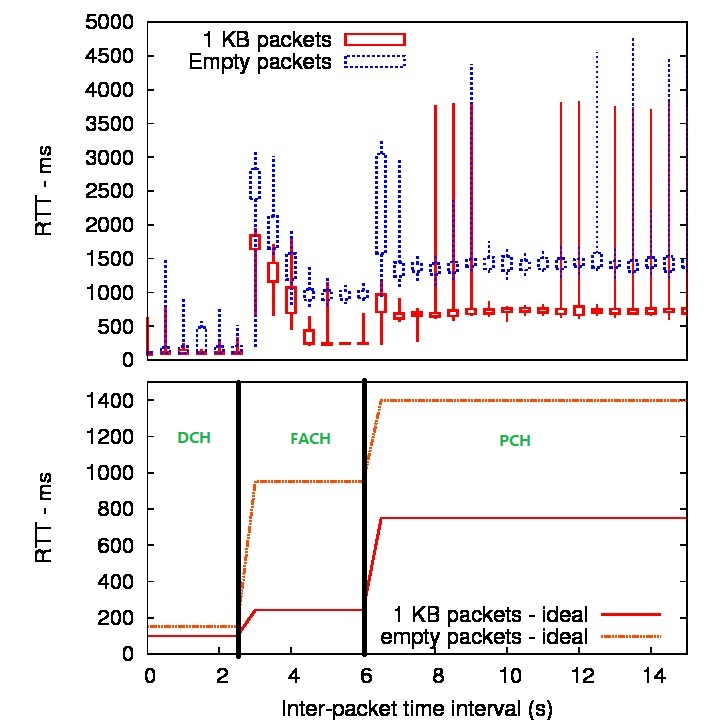
\includegraphics[width=0.5\textwidth]{figs/rrc_inference_result.jpg}
\caption{Reproduced RRC inference algorithm results. Unexpected RTT around inter-packet timing 3.5s.} 
\label{fig:rrc.reproduce}
\end{figure}

~\cite{3g_rrc} tries to infer RRC state using RTT differences. As we mentioned in \S~\ref{subsec:background.rrc}, after the device promoted into DCH state, it could demote to a lower power state, i.e. FACH or PCH, due to timeout on no data transmission. The RRC inference mechanism measures different RTTs based on different inter-packet timing intervals. For any substantial difference in the two adjacent inter-packet timings, we could approximate the demotion timer to be in between the two inter-packet timing intervals. We reproduce results as in Figure~\ref{fig:rrc.reproduce}.

\begin{figure}[t!]
\centering
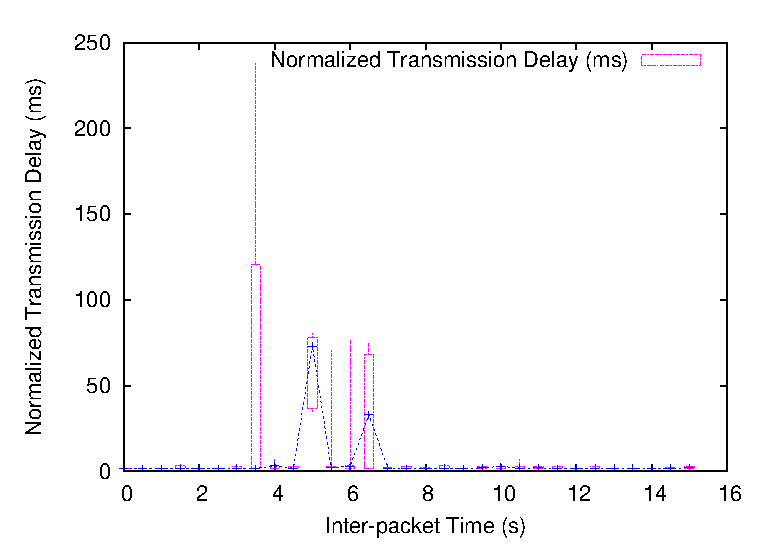
\includegraphics[width=0.5\textwidth]{figs/normalized_transmission_delay.eps}
\caption{In normalized transmission delay feature, we observe the same delay around 3.5s which matches the observation from the \emph{Control Dataset}} 
\label{fig:rlc.normalized.transmission.delay}
\end{figure}

\begin{figure}[t!]
\centering
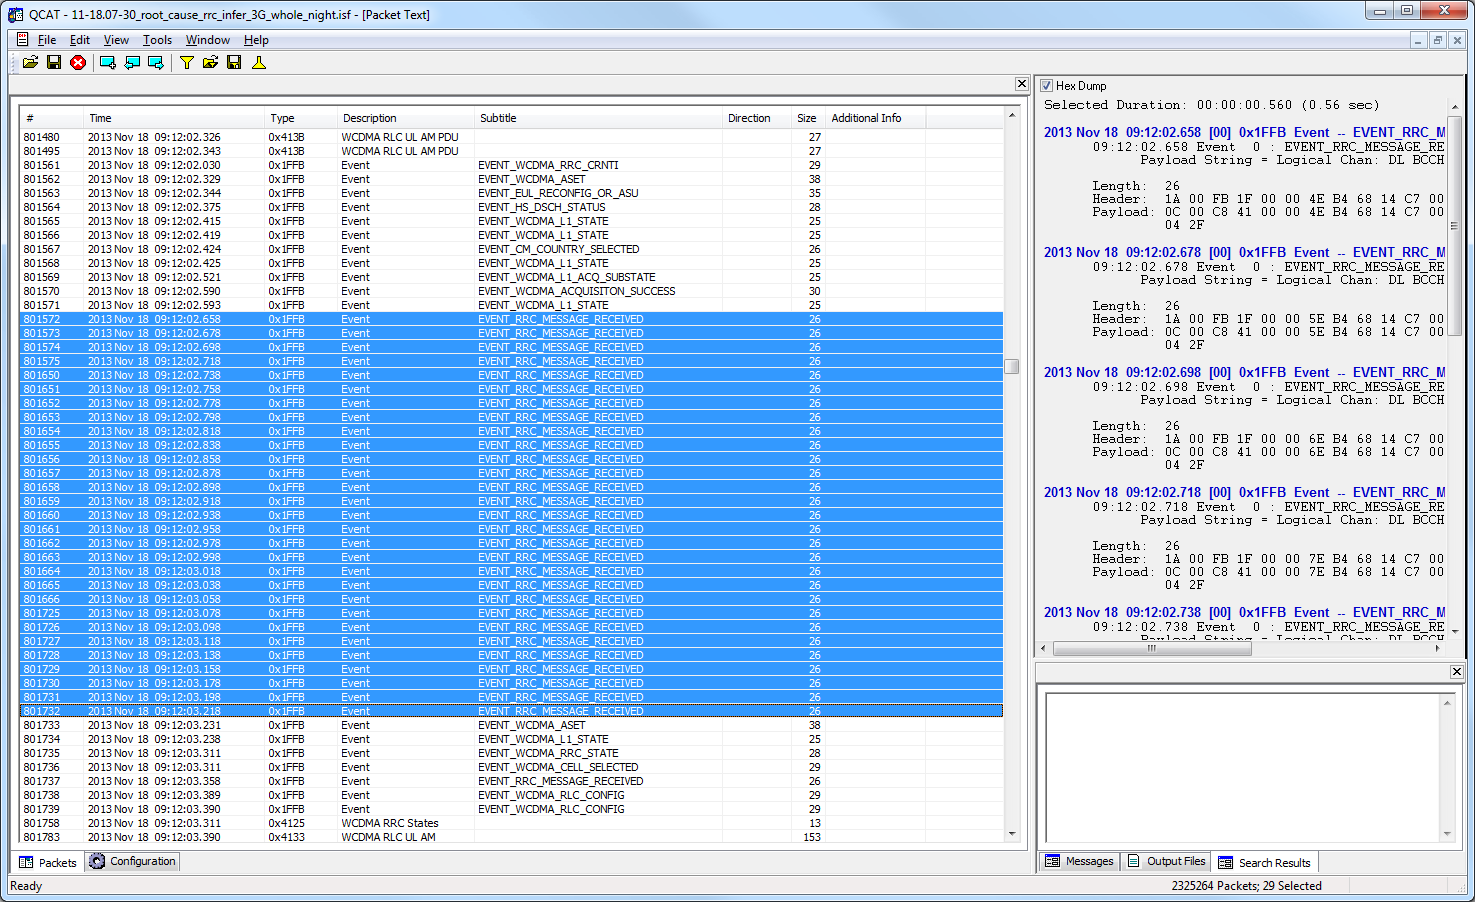
\includegraphics[width=0.5\textwidth]{figs/root_cause_rrc_message_blocking.png}
\caption{QxDM logging information around the inter-packet timing 3.5s. Substantial amount of PRACH control messages from Node B block the data plane transmission} 
\label{fig:qxdm.root.cause}
\end{figure}

We apply the cross-layer mapping, and extract the lower layer features as mentioned in \S~\ref{subsec:lower.layer.features}. Among all the feature, we find the normalized transmission delay matches our control experiments results as in Figure~\ref{fig:rlc.normalized.transmission.delay}. Then we take a deeper dive in the QxDM, we figure out that large amount of control messages arrived in the middle of RLC PDU data transmission as shown in Figure~\ref{fig:qxdm.root.cause}. Data fragmentation as in WCDMA uplink would increase the possibility of unnecessary control message interference. We do not observe similar problems in the downlink because the average PDU size is around 17 times larger than the uplink. That implies much less fragmentation occur in WCDMA downlink, and less chance to get interrupted by control messages.



